\documentclass[conference]{IEEEtran}
\IEEEoverridecommandlockouts
\usepackage[utf8]{inputenc}
\usepackage[T1]{fontenc}
\usepackage{amsmath,amssymb}
\usepackage{graphicx}
\usepackage{booktabs}
\usepackage{multirow}
\usepackage{algorithm}
\usepackage{algpseudocode}
\usepackage{xcolor}
\usepackage{tikz}
\usetikzlibrary{arrows.meta,positioning,fit,calc}
\usepackage[hidelinks]{hyperref}
\usepackage{cite}

\newcommand{\TBD}{\textcolor{red}{\textbf{TBD}}}
\newcommand{\code}[1]{\texttt{#1}}

\begin{document}

\title{Evidence-Grounded Clinical Trial Criterion Matching with a LoRA-Tuned Small Decoder,
KV-Cached and Speculative Decoding, and Tiled Attention}

\author{\IEEEauthorblockN{Mustafa Faraz (23I-0631)\\
\IEEEauthorblockA{Department of Computer Science\\
National University of Computer and Emerging Sciences (FAST-NUCES)\\
Islamabad, Pakistan\\
mustafafaraz87@gmail.com}
}}

\maketitle

\begin{abstract}
Screening patients against free-text clinical-trial eligibility criteria is slow manual work.
We fine-tune the open-weight Qwen2.5-1.5B-Instruct with LoRA on the expert annotations of the
TrialGPT Criterion Annotations dataset to judge one inclusion or exclusion criterion at a time,
returning one of the dataset's four labels per criterion type and the IDs of the supporting patient
sentences. On a patient-disjoint held-out test split, fine-tuning raises accuracy from 0.039 to
0.748, macro-F1 from 0.077 to 0.569 and evidence micro-F1 from 0.095 to 0.513; seed repeats and a
paired bootstrap quantify the variability behind these numbers, and an error analysis shows that
the largest error group stems from inconsistently annotated missing information. We further
implement and verify the inference stack from first principles: a hand-written Qwen2 forward pass
with an explicit pre-allocated KV cache (token-identical to recomputation in fp32, up to
13$\times$ faster on a T4), tiled attention with online softmax (matching exact attention to float
precision with 2.3\,GB less memory at 4,096 tokens, but slower than fused kernels), and greedy
speculative decoding with a fine-tuned 0.5B draft (exact outputs, 93\% acceptance, no speed-up,
which a measured draft/target cost ratio of 0.84 explains). A Dockerized React/FastAPI application
exposes evidence-linked screening, explicit outcome aggregation, report export and live inference
benchmarks on a CPU-only laptop.

\end{abstract}

\begin{IEEEkeywords}
clinical trial matching, eligibility criteria, large language models, LoRA, KV cache,
speculative decoding, FlashAttention, online softmax
\end{IEEEkeywords}

\section{Introduction}
\label{sec:intro}

Clinical trials fail or are delayed far more often for lack of participants than for lack of
scientific merit, and pre-screening patients against free-text eligibility criteria is a laborious
manual step. Each trial lists inclusion and exclusion criteria in natural language; a coordinator must
read a patient's notes and decide, criterion by criterion, whether the patient meets it, does not meet
it, or whether the record simply does not say. Large language models (LLMs) are a natural fit for this
reading task, and TrialGPT~\cite{jin2024trialgpt} showed that GPT-4 can produce criterion-level
judgements with sentence-level evidence that agree well with clinicians.

Relying on a proprietary API is, however, unattractive for patient data and impossible in the
setting of this work, which requires a freely available, locally executable model. This paper
therefore asks how far a \emph{small open-weight decoder} can be pushed on the same task when it is
fine-tuned on the expert annotations released with TrialGPT, and how such a model can be served
efficiently on commodity hardware.

\textbf{Problem statement.} Given a patient note split into numbered sentences, a criterion type
(inclusion or exclusion) and the criterion text, predict (i) one of the dataset's four expert labels
for that criterion type and (ii) the set of patient sentence IDs that support the decision. The
labels deliberately include \emph{not enough information} and \emph{not applicable}; collapsing them
into a binary decision, or treating missing evidence as proof of (in)eligibility, would be unsafe.

\textbf{Contributions.}
\begin{enumerate}
\item A reproducible, leakage-checked pipeline on the TrialGPT Criterion Annotations with the
prescribed patient-grouped 37/8/8 split, and LoRA fine-tuning of Qwen2.5-1.5B-Instruct that raises
held-out accuracy from 0.039 to 0.748 and macro-F1 from 0.077 to 0.569 (Section~\ref{sec:results}).
\item A controlled ablation of answer order, rare-class oversampling and training length, with a
paired bootstrap showing which differences are and are not reliable on a validation set with only a
handful of minority-class examples.
\item A hand-written Qwen2 forward pass with an explicit pre-allocated KV cache, verified to be
token-identical to uncached recomputation and to Hugging Face greedy decoding, extended with prefix
reuse across the criteria of one patient.
\item A tiled attention kernel with online softmax, verified against a float64 reference and PyTorch
SDPA, and usable as a drop-in attention backend of the real model.
\item Greedy speculative decoding with a fine-tuned 0.5B draft model, with cache rollback, verified
token-equivalence and measured acceptance, latency and memory.
\item A Dockerized React/FastAPI screening application that exposes evidence-linked results,
explicit outcome aggregation, report export and live inference benchmarks.
\end{enumerate}

\section{Related Work}
\label{sec:related}

\textbf{Patient--trial matching.} Koopman and Zuccon~\cite{koopman2016test} released the SIGIR 2016
collection of patient case descriptions and candidate trials that underlies the patients in our
dataset; it framed matching as retrieval with graded relevance. TrialGPT~\cite{jin2024trialgpt}
recast the problem as LLM reasoning: GPT-4 first retrieves candidate trials, then judges each
criterion with an explanation and cited patient sentences, and finally aggregates criterion
judgements into a trial-level score. Its criterion-level annotations, in which clinicians labelled
the eligibility of 1,015 patient--criterion pairs and marked the relevant sentences, are the
benchmark used here. TrialGPT's predictions are produced by a proprietary model; we use only the
expert annotations and treat the stored GPT-4 outputs as forbidden inputs. Unlike TrialGPT, which
relies on prompting, we \emph{fine-tune} a model two to three orders of magnitude smaller, trading
general reasoning ability for local execution and task-specific supervision.

\textbf{Transformer decoders.} Our models follow the decoder-only Transformer~\cite{vaswani2017attention}
as refined in Qwen2.5~\cite{qwen2024qwen25}: rotary position embeddings (RoPE)~\cite{su2024roformer},
RMSNorm~\cite{zhang2019rmsnorm}, SwiGLU feed-forward blocks~\cite{shazeer2020glu} and grouped-query
attention (GQA)~\cite{ainslie2023gqa}, which shares each key/value head among several query heads and
shrinks the KV cache proportionally. Llama~3.2~\cite{grattafiori2024llama3} uses the same ingredients
and was our main alternative (Section~\ref{sec:model}).

\textbf{Parameter-efficient adaptation.} LoRA~\cite{hu2022lora} freezes the pretrained weights and
learns a low-rank update $\Delta W = BA$ per adapted matrix, which reduces optimizer state by orders
of magnitude and yields small, separately distributable adapters. QLoRA~\cite{dettmers2023qlora}
additionally quantizes the frozen base to 4 bits; with a 1.5B model the base fits comfortably on a
16\,GB GPU in half precision, so we did not need the quantization and its numerical side effects.

\textbf{Efficient inference.} Autoregressive decoding is memory-bound: each new token needs the
keys and values of all previous tokens. Caching them (the KV cache) turns quadratic recomputation into
linear work; Pope et~al.~\cite{pope2023efficiently} analyse its memory/latency trade-offs, and
PagedAttention~\cite{kwon2023pagedattention} manages it in fixed-size blocks for high-throughput
serving. For attention itself, Milakov and Gimelshein~\cite{milakov2018online} showed that softmax can
be computed in one pass with a running maximum and normalizer; Rabe and Staats~\cite{rabe2021selfattention}
used this to compute attention in $O(\sqrt{n})$ or constant extra memory, and
FlashAttention~\cite{dao2022flashattention} fused the tiled computation into an IO-aware GPU kernel
that never materializes the $n\times n$ score matrix. Speculative decoding~\cite{leviathan2023fast,chen2023accelerating}
lets a small draft model propose several tokens that the target verifies in one forward pass; with
greedy acceptance the output is exactly the target's greedy output, so speed is the only thing at
stake.

\textbf{Limitations of prior approaches for our setting.} Prompted GPT-4 is accurate but not locally
executable; retrieval-style matchers do not produce criterion-level labels or evidence; and
production inference engines (vLLM, FlashAttention kernels) are CUDA-specific and opaque, whereas this
work requires inspectable implementations that also run on a CPU-only laptop. We therefore combine a
small fine-tuned model with educational, verified implementations of the inference techniques above.

\section{Materials and Methods}
\label{sec:methods}

\begin{figure*}[t]
\centering
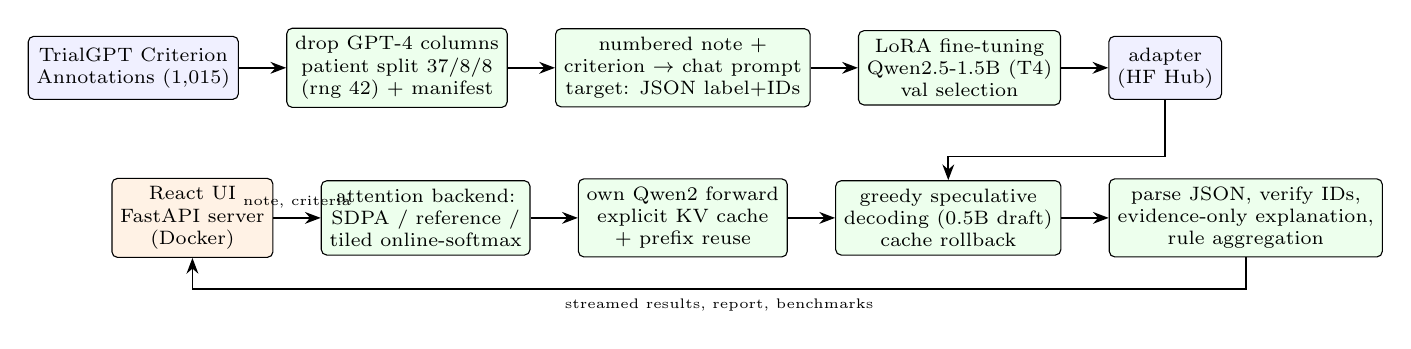
\begin{tikzpicture}[
  node distance=4mm and 6mm,
  box/.style={draw, rounded corners=2pt, align=center, font=\scriptsize, minimum height=8mm, inner sep=3pt},
  data/.style={box, fill=blue!6},
  proc/.style={box, fill=green!7},
  ui/.style={box, fill=orange!10},
  arr/.style={-{Stealth[length=2mm]}, semithick}]
\node[data] (ds) {TrialGPT Criterion\\Annotations (1,015)};
\node[proc, right=of ds] (split) {drop GPT-4 columns\\patient split 37/8/8\\(rng 42) + manifest};
\node[proc, right=of split] (prompt) {numbered note +\\criterion $\rightarrow$ chat prompt\\target: JSON label+IDs};
\node[proc, right=of prompt] (lora) {LoRA fine-tuning\\Qwen2.5-1.5B (T4)\\val selection};
\node[data, right=of lora] (adapter) {adapter\\(HF Hub)};
\node[proc, below=9mm of prompt] (dec) {own Qwen2 forward\\explicit KV cache\\+ prefix reuse};
\node[proc, left=of dec] (attn) {attention backend:\\SDPA / reference /\\tiled online-softmax};
\node[proc, right=of dec] (spec) {greedy speculative\\decoding (0.5B draft)\\cache rollback};
\node[proc, right=of spec] (post) {parse JSON, verify IDs,\\evidence-only explanation,\\rule aggregation};
\node[ui, left=of attn] (ui) {React UI\\FastAPI server\\(Docker)};
\draw[arr] (ds) -- (split);
\draw[arr] (split) -- (prompt);
\draw[arr] (prompt) -- (lora);
\draw[arr] (lora) -- (adapter);
\draw[arr] (adapter) |- ($(spec.north)+(0,3mm)$) -- (spec.north);
\draw[arr] (attn) -- (dec);
\draw[arr] (dec) -- (spec);
\draw[arr] (spec) -- (post);
\draw[arr] (ui) -- node[above, font=\tiny]{note, criteria} (attn);
\draw[arr] (post.south) -- ++(0,-4mm) -| node[pos=0.25, below, font=\tiny]{streamed results, report, benchmarks} (ui.south);
\end{tikzpicture}
\caption{System overview. Top: data preparation and supervised adaptation. Bottom: the inference
stack used by the application, built on our own decoder, attention and decoding implementations.}
\label{fig:overview}
\end{figure*}

Fig.~\ref{fig:overview} summarizes the system: the upper row prepares the data and adapts the model,
the lower row is the inference stack used for evaluation benchmarks and by the application.

\subsection{Dataset and split}
\label{sec:data}
The TrialGPT Criterion Annotations~\cite{jin2024trialgpt} contain 1,015 patient--criterion pairs
from 53 SIGIR-2016 patients~\cite{koopman2016test} and 103 trials. Each record holds the patient
note, already split into numbered sentences (3--14 per note, at most 235 words), the criterion type
and text, the expert eligibility label and the expert evidence sentence IDs. The record also stores
GPT-4's label, explanation and cited sentences, a judgement of that explanation
(\code{explanation\_correctness}) and the original authors' own \code{training} flag. All five fields
are removed when the dataset is loaded, so they cannot reach a prompt, a target or a metric.

The split follows the assignment protocol exactly: the 53 unique patient IDs are sorted,
shuffled with \code{numpy.random.default\_rng(42)}, and the first 37 go to training, the next 8 to
validation and the last 8 to testing. Every annotation of a patient therefore lives in exactly one
split; the preparation script asserts disjoint patient sets, single assignment of every annotation
and absence of leaky fields, and writes a manifest with patient IDs and label counts.
Table~\ref{tab:split} shows the resulting distribution. The label distribution is heavily skewed:
\emph{not excluded} accounts for almost half of all records, while \emph{excluded} occurs only 10
times overall and \emph{not at all} in the test split. One training annotation (ID 883) has an empty
criterion text; it remains assigned to its patient's split in the manifest but is excluded from
training because no task can be posed for it.

\begin{table}[t]
\centering
\caption{Patient-grouped split (seed 42) and label distribution.}
\label{tab:split}
\setlength{\tabcolsep}{4pt}
\begin{tabular}{llrrr}
\toprule
 & & Train & Val & Test \\
\midrule
\multicolumn{2}{l}{Patients} & 37 & 8 & 8 \\
\multicolumn{2}{l}{Annotations (used)} & 602 & 206 & 206 \\
\multicolumn{2}{l}{\quad with gold evidence} & 254 & 90 & 61 \\
\midrule
\multirow{4}{*}{Inclusion} & included & 88 & 35 & 27 \\
 & not included & 13 & 3 & 7 \\
 & not enough information & 109 & 27 & 38 \\
 & not applicable & 5 & 1 & 3 \\
\midrule
\multirow{4}{*}{Exclusion} & excluded & 8 & 2 & 0 \\
 & not excluded & 291 & 101 & 91 \\
 & not enough information & 65 & 26 & 28 \\
 & not applicable & 23 & 11 & 12 \\
\bottomrule
\end{tabular}
\end{table}

\subsection{Input/output format and tokenization}
\label{sec:format}
Each example becomes a two-turn chat in the model's template: a system message that frames the task
and states that missing information is never proof of eligibility or ineligibility, and a user
message with the numbered note, the criterion type, the criterion text, a one-line definition of each
of the four labels for that criterion type, and the required output schema. The target is a single
JSON object, e.g.\ \code{\{"label": "included", "evidence": [0, 3]\}}, followed by the end-of-turn
token. The four label sets are kept separate for inclusion and exclusion criteria, so the model always
chooses among the labels that are valid for the given type.

With the Qwen2.5 tokenizer (byte-level BPE, 151,665 tokens) prompts are 256--625 tokens long and
targets 12--38 tokens; the longest prompt plus target is 651 tokens. We therefore set the maximum
sequence length to 768, which means \emph{no example is truncated}. The training code raises an error
instead of truncating, and the application rejects (with a clear message) any input above 2,048
tokens, because silently cutting the note could remove exactly the evidence a decision depends on.

Generated text is parsed by extracting the first JSON object; a label outside the type's label set is
invalid, and cited IDs that do not exist in the note are discarded. If the JSON is malformed but a
valid label string appears, the label is recovered and the record is flagged.

\subsection{Model selection}
\label{sec:model}
Table~\ref{tab:models} compares the candidates we considered. All are decoder-only Transformers with
RoPE, RMSNorm, SwiGLU and GQA, so all support the required KV-cache and speculative-decoding work. Two
constraints dominated the choice: LoRA training must fit one free 16\,GB T4 GPU, and the application
must run on a CPU-only laptop with 16\,GB RAM. Speculative decoding additionally requires a smaller
model with an \emph{identical tokenizer}.

\begin{table}[t]
\centering
\caption{Candidate open-weight decoders (values from the model configurations).}
\label{tab:models}
\setlength{\tabcolsep}{2.5pt}
\begin{tabular}{lcccc}
\toprule
 & Qwen2.5 & Qwen2.5 & Llama 3.2 & Llama 3.2 \\
 & 1.5B-Instr. & 0.5B-Instr. & 1B-Instr. & 3B-Instr. \\
\midrule
Parameters & 1.54B & 0.49B & 1.24B & 3.21B \\
Layers / hidden & 28 / 1536 & 24 / 896 & 16 / 2048 & 28 / 3072 \\
Q / KV heads & 12 / 2 & 14 / 2 & 32 / 8 & 24 / 8 \\
Head dim & 128 & 64 & 64 & 128 \\
Vocabulary & 151,936 & 151,936 & 128,256 & 128,256 \\
Context & 32K & 32K & 128K & 128K \\
KV cache / token (fp16) & 28\,KB & 12\,KB & 32\,KB & 112\,KB \\
Weights fp16 / fp32 & 3.1 / 6.2\,GB & 1.0 / 2.0\,GB & 2.5 / 5.0\,GB & 6.4 / 12.8\,GB \\
License & Apache-2.0 & Apache-2.0 & Llama 3.2 & Llama 3.2 \\
\bottomrule
\end{tabular}
\end{table}

We selected \textbf{Qwen2.5-1.5B-Instruct} as the target and \textbf{Qwen2.5-0.5B-Instruct} as the
draft. The pair shares one tokenizer and chat template, is Apache-2.0 licensed with ungated downloads,
and the target's aggressive GQA (12 query heads, 2 KV heads) gives the smallest KV cache per token of
the larger candidates. Its fp32 weights (6.2\,GB) fit the laptop's RAM for CPU inference, whereas
Llama~3.2-3B (12.8\,GB in fp32) does not leave room for the draft, the cache and the OS. The
Llama~3.2-1B/3B pair was a viable alternative; we rejected it because of the gated license, the
larger KV cache of the 3B model, and because a 1B target would leave too little room between target
and draft for speculative decoding to pay off.

\subsection{Supervised fine-tuning}
\label{sec:finetune}
We adapt all seven linear projections of every layer ($W_q, W_k, W_v, W_o$ and the gate, up and down
projections of the MLP) with LoRA~\cite{hu2022lora}: $W' = W + \frac{\alpha}{r}BA$ with rank $r=16$,
$\alpha=32$ and dropout 0.05, i.e.\ 18.5M trainable parameters (1.18\%). The objective is the causal
language-modelling cross-entropy on the \emph{answer tokens only}; prompt positions are masked with
$-100$ so the model is not trained to reproduce notes or criteria. The frozen base weights are loaded
in fp16 (the T4 has no native bf16), adapters are kept in fp32, and training uses automatic mixed
precision with dynamic loss scaling.

The training loop is written in plain PyTorch rather than with a trainer abstraction: AdamW,
learning rate $2\cdot10^{-4}$ with 5\% linear warm-up and cosine decay, gradient clipping at 1.0,
micro-batch 2 with 4 accumulation steps (effective batch 8), 3 epochs, seed 42. A micro-batch of 4
ran out of GPU memory: with a 151,936-word vocabulary the fp32 logits of a single micro-batch of four
651-token sequences occupy $4\cdot651\cdot151{,}936\cdot4$\,B $\approx$ 1.6\,GB, and several copies
exist during the loss and backward computation. Gradient checkpointing keeps the peak at 5.5\,GB.
After every epoch the adapter is saved, the teacher-forced validation loss is computed, and the
validation split is decoded greedily and scored; the epoch with the highest validation macro-F1 is
kept. The test split is read only by the final evaluation command (Section~\ref{sec:setup}).

\textbf{Ablations.} Three alternatives were trained with otherwise identical settings and compared on
validation only: (i) \emph{label-first} answer order versus the \emph{evidence-first} order of our
initial design, which asks the model to commit to evidence before the label; (ii) \emph{rare-class
oversampling}, which repeats every training example $\min(8,\operatorname{round}(\sqrt{n_{\max}/n_c}))$
times per epoch, where $n_c$ is the count of its (criterion type, label) class (602 $\rightarrow$
1,060 examples per epoch); (iii) training for 5 instead of 3 epochs. The 0.5B draft model is
fine-tuned with the same recipe and the selected answer order.

\subsection{Explicit KV-cached decoding}
\label{sec:kv}
To control every step of cached decoding we implemented the Qwen2 forward pass ourselves on top of
the trained weight tensors (embedding, projections, norms); only the linear layers are reused as
modules. Per layer: $x \leftarrow h + W_o\,\mathrm{Attn}(\mathrm{RoPE}(W_q\bar h + b_q),
\mathrm{RoPE}(W_k\bar h + b_k), W_v\bar h + b_v)$ with $\bar h = \mathrm{RMSNorm}(h)$, followed by
$h \leftarrow x + W_d(\mathrm{SiLU}(W_g\bar x)\odot W_u\bar x)$.

\textbf{Cache layout and growth.} The cache holds, for each of the 28 layers, a key and a value
tensor of shape $(B, H_{kv}{=}2, L_{\max}, 128)$ that is \emph{pre-allocated} for the prompt length
plus the generation budget; a single integer \code{length} marks the valid prefix. A forward call on
$T$ new tokens at absolute position $p$ writes their keys and values into slots $p\ldots p{+}T{-}1$
and attends over slots $0\ldots p{+}T{-}1$. Growth therefore costs $O(1)$ per token instead of the
$O(n)$ reallocation of repeated concatenation, and rollback (needed by speculative decoding and by
prefix reuse) is just lowering \code{length}. Memory grows linearly: $2 \cdot 28 \cdot 2 \cdot 128$
values, i.e.\ 28\,KB per token in fp16. Keys and values are stored with the 2 KV heads and expanded to
the 12 query heads only inside attention, so GQA's 6$\times$ saving is kept.

\textbf{Positional handling.} RoPE rotates queries and keys by angles $\theta_i\,m$ that depend on
the absolute position $m$; cached keys were rotated when they were written. New tokens must therefore
be rotated with $m = p, \ldots, p{+}T{-}1$ rather than $0\ldots T{-}1$, otherwise their relative
offsets to the cached keys would be wrong. Our forward pass takes $p$ explicitly and computes
$\cos/\sin$ tables for exactly those positions (base $\theta = 10^6$).

\textbf{Masking.} With $T$ new queries and $p+T$ keys, query $i$ may attend key $j$ iff
$j \le i + p$: a causal mask aligned to the \emph{bottom-right} of the $T\times(p{+}T)$ score matrix.
PyTorch's \code{is\_causal} flag aligns to the top-left, which is only correct when $p=0$; we pass the
bottom-right mask explicitly when $p>0$ and $T>1$. For single-token decode steps ($T=1$) no mask is
needed because every cached position is in the past.

\textbf{Prefix reuse.} In the application all criteria of one patient share the system prompt and
the note. The cache remembers which token IDs its valid slots belong to; a new prompt reuses the
longest common token prefix (keeping at least one token to produce logits), crops the rest, and
prefills only the new suffix.

\textbf{Reference path and numerics.} The uncached reference allocates a fresh cache and runs the
full sequence at every step, i.e.\ $O(n^2)$ total work for $n$ tokens. In exact arithmetic both paths
compute the same logits. In floating point they need not be bitwise identical: the cached path
computes the new token's projections as a $1\times d$ product while the reference computes them as one
row of a $T\times d$ product, and different matrix shapes select different kernels and summation
orders. Differences are of the order of float rounding and can flip a greedy argmax only when the top
two logits are within that margin, which we test for explicitly (Section~\ref{sec:res-kv}).

\subsection{Tiled attention with online softmax}
\label{sec:tiled}
The reference attention computes $S = QK^\top/\sqrt{d}$, applies the mask with $-\infty$, subtracts
the row maximum before exponentiation and normalizes; it materializes the full $L_q\times L_k$ score
matrix. The tiled variant (Algorithm~\ref{alg:tiled}) processes queries in blocks of $B_q$ rows and
streams over key/value blocks of $B_k$ columns, keeping per row a running maximum $m$, a running
normalizer $\ell$ and an unnormalized output accumulator $o$~\cite{milakov2018online,dao2022flashattention}.
When a new block raises the maximum, previous contributions are rescaled by $e^{m-m'}$, so the result
is exactly softmax-weighted, while only a $B_q\times B_k$ tile of scores exists at any time. Under
causal masking, key blocks entirely above the diagonal are skipped. Half-precision inputs are
accumulated in fp32. Rows whose blocks are fully masked keep $m=-\infty$, so the subtraction uses a
safe maximum of 0 to avoid $-\infty-(-\infty)$.

\begin{algorithm}[t]
\caption{Tiled attention with online softmax (one query block)}
\label{alg:tiled}
\begin{algorithmic}[1]
\Require $Q_b\in\mathbb{R}^{B_q\times d}$, $K, V\in\mathbb{R}^{L_k\times d}$, scale $s$, mask
\State $m \gets -\infty^{B_q}$, $\ell \gets 0^{B_q}$, $o \gets 0^{B_q\times d}$
\For{each key block $j$ (skipping blocks above the causal diagonal)}
  \State $S \gets s\,Q_b K_j^\top$; set masked entries of $S$ to $-\infty$
  \State $m' \gets \max(m, \operatorname{rowmax}(S))$
  \State $P \gets \exp(S - m')$; \quad $c \gets \exp(m - m')$
  \State $\ell \gets c\odot\ell + \operatorname{rowsum}(P)$; \quad $o \gets c\odot o + P V_j$
  \State $m \gets m'$
\EndFor
\State \Return $o / \ell$
\end{algorithmic}
\end{algorithm}

Both kernels are registered as attention backends of the Hugging Face model
(\code{attn\_implementation="tiled"}), and our decoder can select them. Registering only the attention
function is not enough: the library then passes \emph{no} attention mask to an unknown backend, so a
left-padded batch silently attends to padding tokens (we measured logit errors up to 10.6). Registering
the SDPA mask builder under the same name fixes this.

\subsection{Greedy speculative decoding}
\label{sec:spec}
Algorithm~\ref{alg:spec} gives our greedy variant of speculative decoding~\cite{leviathan2023fast,chen2023accelerating}.
Both models keep their own KV cache with the invariant that, between iterations, each cache holds
every committed token except the last one, which is the pending input. In an iteration the draft first
catches up on committed tokens it has not processed, then proposes $k$ tokens greedily. The target
processes the last committed token and the $k$ drafts in \emph{one} forward pass; row $i$ of its
logits is the target's greedy choice after drafts $1\ldots i$. The longest prefix of drafts matching
the target's choices is accepted, and the target's own token at the first mismatch (or a bonus token
if all match) is appended, so every iteration commits between 1 and $k{+}1$ tokens. Finally both
caches are cropped to the committed length minus one, discarding the keys and values of rejected
drafts. Because every committed token equals the target's argmax given the committed prefix, the
output is identical to plain greedy decoding of the target.

\begin{algorithm}[t]
\caption{Greedy speculative decoding}
\label{alg:spec}
\begin{algorithmic}[1]
\Require prompt $x$, target $M_t$, draft $M_d$, draft length $k$
\State prefill $M_t$ on $x$; $y \gets x \,\|\, \arg\max M_t(x)$
\While{budget left and last token $\neq$ EOS}
  \State $M_d$: feed $y[\text{len}(C_d):]$, then draft $d_1..d_k$ greedily
  \State $M_t$: one pass on $[y_{-1}, d_1..d_k]$ $\rightarrow$ choices $g_0..g_k$
  \State $n \gets$ largest $n$ with $d_i = g_{i-1}\;\forall i\le n$
  \State $y \gets y \,\|\, d_1..d_n \,\|\, g_n$ \Comment{truncate at EOS / budget}
  \State crop $C_t$ and $C_d$ to $|y| - 1$
\EndWhile
\end{algorithmic}
\end{algorithm}

\subsection{Explanations, aggregation and application}
\label{sec:app}
The dataset contains no expert explanations, so the model is not trained to write free text.
Instead, each prediction's explanation is assembled \emph{only} from the cited sentences (quoted with
their IDs) and the meaning of the predicted label; a decisive label without cited evidence is flagged
\emph{unsupported}, and \emph{not enough information} lists the criterion as missing information.
This avoids hallucinated rationales at the cost of fluency. The overall patient--trial outcome is
an explicit rule, not a learned or ground-truth label: \emph{likely ineligible} if any inclusion
criterion is \emph{not included} or any exclusion criterion is \emph{excluded}; otherwise \emph{needs
clinician review} if any criterion has insufficient information or could not be parsed; otherwise
\emph{potentially eligible}.

The application (Fig.~\ref{fig:overview}, bottom) is a FastAPI server with a React front end,
packaged as a Docker image and started with one command. The user pastes a note (or loads a
validation example), enters or pastes criteria or fetches them from ClinicalTrials.gov by NCT ID,
chooses a decoding mode and runs the screening. Results stream back criterion by criterion with the
label, evidence sentences highlighted in the numbered note, explanation, flags and timing. Reports are
saved with provenance (model, adapter, decoding settings, time) and can be downloaded as HTML or JSON.
A benchmark page runs a chosen prompt live through the uncached, cached, tiled-attention and
speculative decoders and shows timings, token equality and draft acceptance, and an experiments page
renders training curves, confusion matrices and GPU benchmarks from the logged result files.

\section{Experimental Setup and Metrics}
\label{sec:setup}

\textbf{Hardware and software.} Training, evaluation and GPU benchmarks ran as non-interactive
Kaggle script jobs on one NVIDIA Tesla T4 (15\,GB usable, fp16, no bf16), PyTorch~2.11 (CUDA~12.8),
Transformers~5.20 and PEFT~0.21. Each job clones the repository at a recorded commit, runs, and
exits so the GPU is released immediately; a short preflight on the longest examples precedes every
training run so that environment or memory errors cost seconds rather than minutes. The application
and the CPU measurements ran on a laptop with an Intel Core i5-1135G7 (4 cores) and 16\,GB RAM,
PyTorch~2.14 (CPU) in fp32. In total all GPU experiments used \TBD{} of the free 30-hour weekly quota.

\textbf{Decoding settings.} All reported predictions use greedy decoding (argmax), at most 64 new
tokens, batch size 16 for evaluation, and \code{repetition\_penalty}$=1.0$. The latter matters:
Qwen's shipped generation configuration enables sampling and a repetition penalty of 1.1, and the
library applies the penalty even when sampling is disabled. We found this when our own decoder
disagreed with library greedy decoding at the third token; with the penalty disabled the two agree
token for token. The zero-shot baseline and the fine-tuned model use the identical prompt, examples
and decoding settings.

\textbf{Classification metrics.} We report accuracy, macro-F1, per-class precision, recall and F1, and
confusion matrices, overall and separately for inclusion and exclusion criteria. Unparseable outputs
count as a separate \emph{invalid} prediction and are always wrong. Macro-F1 averages over the gold
classes present in the evaluated subset; a class with no gold examples (e.g.\ \emph{excluded} in the
test split) has undefined recall and is reported but not averaged, rather than being silently scored
as 0 or 1. Because the overall label space merges the two criterion types, the shared labels
(\emph{not enough information}, \emph{not applicable}) form single classes in the overall figures.

\textbf{Evidence metrics.} Predictions and gold annotations are sets of original sentence IDs.
\emph{Micro} precision/recall/F1 sum true positives, false positives and false negatives over all
records; records with an empty gold set contribute every predicted ID as a false positive.
\emph{Macro} scores average per-record precision, recall and F1 over records with a \emph{non-empty}
gold set (precision is 0 when nothing is predicted). For the 56--70\% of records whose gold set is
empty we report \emph{empty-gold agreement}: the fraction where the model also cites nothing. Absent
evidence is never interpreted as a label.

\textbf{Statistical comparison.} Ablations are compared with a paired bootstrap over validation
annotations (2,000 resamples): for each resample we compute the metric difference between a variant
and the main run, and report the mean difference, its 95\% percentile interval and the fraction of
resamples in which the variant is better.

\textbf{Timing protocol.} Benchmarks use batch size 1 and the same model, weights and inputs for every
mode. Each configuration is run once for warm-up and then repeated (3 times for decoding, 10 for
attention); we report the median. CUDA is synchronized before every clock read, so asynchronous
kernel launches cannot hide work. \emph{Prefill} time is measured up to the first generated token
(including the first argmax), \emph{decode} time covers the remaining tokens, and tokens/s is output
tokens divided by total time. Peak memory is the CUDA allocator peak after resetting its statistics.
For fixed-length comparisons the end-of-sequence token is ignored so every mode generates the same
number of tokens.

\section{Results and Discussion}
\label{sec:results}

\subsection{Fine-tuning: before and after}
\label{sec:res-ft}

Table~\ref{tab:main} compares the untuned Qwen2.5-1.5B-Instruct with the selected LoRA model on
identical validation and test examples, with the identical label-first prompt and greedy decoding.
Fine-tuning raises held-out test accuracy from 0.039 to \textbf{0.748}, macro-F1 from 0.077 to
\textbf{0.569} and evidence micro-F1 from 0.095 to \textbf{0.513}; every output of both models
was valid JSON with a valid label, so the gains are not a formatting artefact. The zero-shot model
is degenerate under this prompt: it answers \emph{excluded} for every validation exclusion criterion
and \emph{not applicable} for almost every inclusion criterion. With the evidence-first prompt the
same untuned model reaches 0.209 accuracy (macro-F1 0.142) on validation, still mostly answering
\emph{excluded}, i.e.\ confusing ``the note is about the excluded condition'' with ``the patient has
it''. The untuned model is thus highly prompt-sensitive, and asking it to cite evidence first helps
it, whereas after fine-tuning the answer order barely matters (Section~\ref{sec:res-abl}).

\begin{table}[t]
\centering
\caption{Before/after fine-tuning (label-first prompt, greedy). Ev.\ = evidence;
empty = agreement on records with no gold evidence.}
\label{tab:main}
\setlength{\tabcolsep}{3pt}
\begin{tabular}{llcccccc}
\toprule
 & & \multicolumn{2}{c}{Label} & \multicolumn{2}{c}{Ev.\ micro} & Ev.\ macro & Ev.\ \\
Split & Model & Acc & M-F1 & P & F1 & F1 & empty \\
\midrule
\multirow{2}{*}{Val} & zero-shot & 0.015 & 0.009 & 0.043 & 0.075 & 0.119 & 0.138 \\
 & LoRA & 0.743 & 0.544 & 0.504 & 0.551 & 0.606 & 0.836 \\
\midrule
\multirow{2}{*}{Test} & zero-shot & 0.039 & 0.077 & 0.054 & 0.095 & 0.138 & 0.207 \\
 & LoRA & \textbf{0.748} & \textbf{0.569} & 0.439 & \textbf{0.513} & 0.606 & 0.869 \\
\midrule
\multicolumn{8}{l}{\emph{Test by criterion type (LoRA)}} \\
 & inclusion & 0.773 & 0.417 & 0.466 & 0.582 & 0.686 & 0.633 \\
 & exclusion & 0.733 & 0.521 & 0.345 & 0.328 & 0.381 & 0.930 \\
\bottomrule
\end{tabular}
\end{table}

Fig.~\ref{fig:cm} and Table~\ref{tab:perclass} break the test result down. The model is reliable on
the frequent classes (F1 0.83--0.84 for \emph{included}, \emph{not excluded} and inclusion
\emph{not enough information}) and on exclusion \emph{not applicable} (precision 0.75). It never
predicts the rare inclusion classes: all seven \emph{not included} and all three \emph{not
applicable} inclusion cases are answered \emph{not enough information} (six) or \emph{included}
(one). Its weakest class is exclusion \emph{not enough information} (recall 0.07): 25 of 28 such
criteria are predicted \emph{not excluded}. Overall accuracy therefore overstates performance on
the decisions that matter most; macro-F1, which weighs every class equally, is the more honest
summary. Inclusion criteria have higher accuracy but lower macro-F1 than exclusion criteria
because the two zero-recall classes are both inclusion classes.

\begin{figure*}[t]
\centering
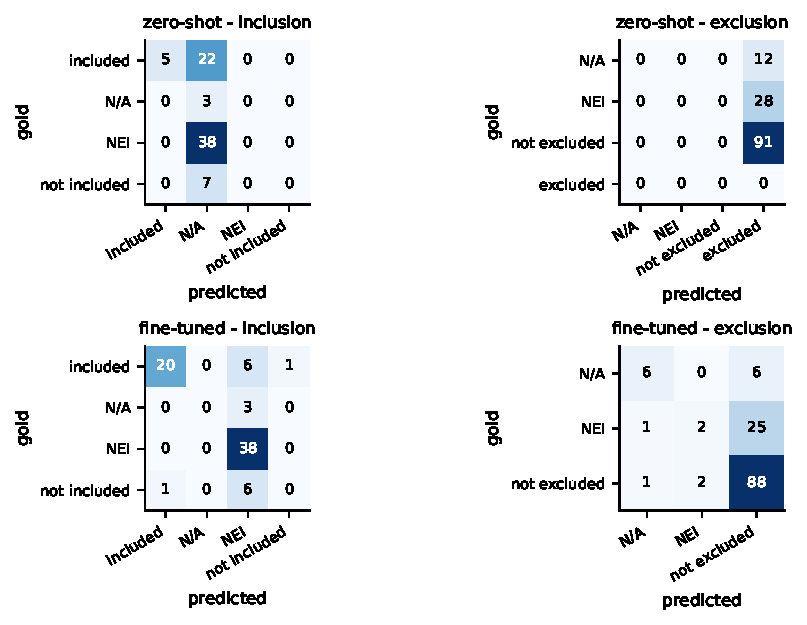
\includegraphics[width=0.8\textwidth]{figures/confusion_test}
\caption{Test confusion matrices (rows gold, columns predicted) for the zero-shot (top) and
fine-tuned (bottom) model, inclusion (left) and exclusion (right). The test split has no
\emph{excluded} example.}
\label{fig:cm}
\end{figure*}

\begin{table}[t]
\centering
\caption{Per-class test metrics of the final model.}
\label{tab:perclass}
\setlength{\tabcolsep}{4pt}
\begin{tabular}{llcccr}
\toprule
Type & Class & P & R & F1 & n \\
\midrule
\multirow{4}{*}{Inclusion} & included & 0.95 & 0.74 & 0.83 & 27 \\
 & not included & 0.00 & 0.00 & 0.00 & 7 \\
 & not enough information & 0.72 & 1.00 & 0.84 & 38 \\
 & not applicable & 0.00 & 0.00 & 0.00 & 3 \\
\midrule
\multirow{4}{*}{Exclusion} & excluded & -- & -- & -- & 0 \\
 & not excluded & 0.74 & 0.97 & 0.84 & 91 \\
 & not enough information & 0.50 & 0.07 & 0.13 & 28 \\
 & not applicable & 0.75 & 0.50 & 0.60 & 12 \\
\bottomrule
\end{tabular}
\end{table}

\textbf{Evidence.} When the gold evidence set is non-empty the model recovers 62\% of the gold
sentences (micro recall 0.617) at precision 0.44; per-record macro-F1 is 0.61. On the 145 test
records without gold evidence it correctly cites nothing in 87\% of cases. Evidence precision is
lowest for exclusion criteria (0.35), where the model tends to cite every symptom sentence of a
note when it judges a criterion. Even when the label is correct, the cited set differs from the
expert set in 36 of 154 correct predictions, often by citing one plausible extra sentence.

\textbf{Seed variability and reproducibility.} Retraining the final recipe with seeds 43 and 44
gives validation macro-F1 $0.554 \pm 0.008$ and test macro-F1 $0.551 \pm 0.017$ (mean $\pm$ s.d.\
over seeds 42--44; test accuracy $0.738 \pm 0.013$, evidence micro-F1 $0.544 \pm 0.036$), so the
reported model is representative rather than a lucky run. The published adapter, downloaded from
the Hugging Face Hub and run in fp32 on the laptop CPU, reproduced the Kaggle T4 fp16 outputs
character for character on 40 of 40 validation examples.

\subsection{Training dynamics and ablations}
\label{sec:res-abl}

Fig.~\ref{fig:curves} shows the training loss (answer tokens only) and validation macro-F1 per epoch
for all variants; Table~\ref{tab:ablation} summarizes them. Training loss falls by an order of
magnitude in the first epoch and keeps decreasing, while teacher-forced validation loss is flat
after epoch 1--2 (0.13--0.15), so longer training mainly sharpens already-learned outputs: five
epochs reach the best evidence F1 (0.577) but not a better macro-F1. Oversampling drives the
training loss down to $\approx$0.005 by memorizing the repeated rare examples, and its validation
macro-F1 peaks after one epoch and then declines, a textbook overfitting pattern. It does shift
recall towards minority classes (validation \emph{included} 23$\rightarrow$32 of 35, exclusion
\emph{not enough information} 7$\rightarrow$13 of 26) at the expense of \emph{not excluded}
(95$\rightarrow$82 of 101).

\begin{figure*}[t]
\centering
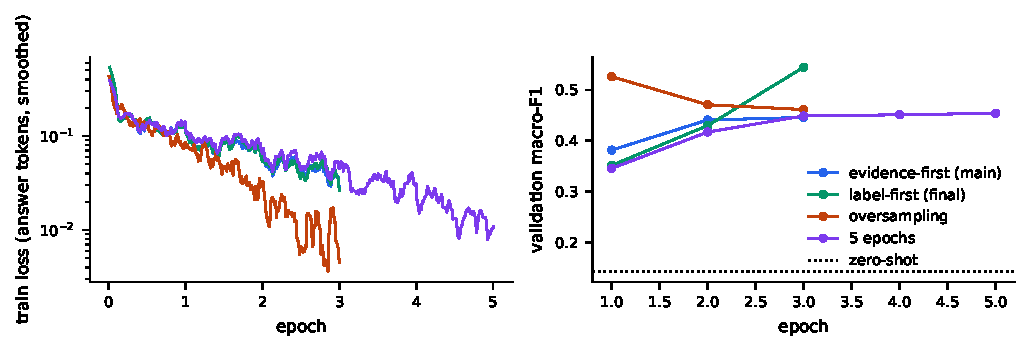
\includegraphics[width=0.85\textwidth]{figures/training_curves}
\caption{Left: training loss on answer tokens (moving average, log scale) per epoch. Right:
validation macro-F1 after each epoch; the dotted line is the evidence-first zero-shot baseline.}
\label{fig:curves}
\end{figure*}

\begin{table}[t]
\centering
\caption{Validation ablations (best epoch by validation macro-F1) and paired-bootstrap
difference in macro-F1 vs.\ the evidence-first main run (95\% interval).}
\label{tab:ablation}
\setlength{\tabcolsep}{2.5pt}
\begin{tabular}{lccccc}
\toprule
Variant (epoch) & Acc & M-F1 & Ev.\ F1 & $\Delta$M-F1 [95\% CI] & T4 s \\
\midrule
evidence-first (3) & 0.748 & 0.446 & 0.544 & -- & 810 \\
label-first (3) & 0.743 & \textbf{0.545} & 0.551 & +0.069 [$-$0.030, 0.168] & 822 \\
oversampling (1) & 0.738 & 0.526 & 0.489 & +0.063 [$-$0.031, 0.177] & 1290 \\
5 epochs (5) & 0.752 & 0.454 & 0.577 & +0.008 [$-$0.015, 0.033] & 1378 \\
\midrule
0.5B, label-first (2) & 0.748 & 0.447 & 0.486 & \multicolumn{2}{l}{(draft model)} \\
\bottomrule
\end{tabular}
\end{table}

No variant is reliably better than the main run: every bootstrap interval for accuracy, macro-F1
and evidence F1 contains zero, and oversampling lowers evidence F1 in 95\% of resamples. The
validation split contains only three \emph{not included}, two \emph{excluded} and one inclusion
\emph{not applicable} example, so a single extra correct rare-class prediction moves macro-F1 by
$\approx$0.1; label-first's lead is exactly one additional correct \emph{excluded}. We nevertheless
kept the selection rule fixed in advance (best validation macro-F1) and chose label-first, and the
seed study above shows that this configuration is stable. The fine-tuned 0.5B draft reaches 0.748
validation accuracy itself, which explains its high draft acceptance (Section~\ref{sec:res-spec}).

\subsection{Error analysis}
\label{sec:res-err}

The final model makes 52 label errors on the 206 test criteria. Table~\ref{tab:errors} lists
representative cases, grouped into the failure modes we observed.

\begin{table*}[t]
\centering
\caption{Representative test errors of the final model (annotation ID, criterion type; gold vs.\
predicted label with cited sentence IDs).}
\label{tab:errors}
\footnotesize
\setlength{\tabcolsep}{3pt}
\begin{tabular}{p{0.45cm}p{3.1cm}p{4.6cm}p{3.0cm}p{5.2cm}}
\toprule
ID & Criterion & Relevant note content & Gold $\rightarrow$ predicted & Failure mode \\
\midrule
186 & (I) Heart rate of at least 90/min & [2] ``\ldots tachypneic and tachycardic.'' & included [2] $\rightarrow$ NEI [3] & \emph{Under-inference}: qualitative term (tachycardic) not mapped to the numeric threshold. \\
187 & (I) Respiratory rate $\ge$ 20/min or \ldots & [2] same sentence & included [2] $\rightarrow$ NEI [2] & Cites the right sentence but refuses the inference. \\
382 & (I) $\ge$4 ACR criteria for SLE & [0--2] arthralgia, malar rash, alopecia, anemia, thrombocytopenia, ANA, anti-dsDNA & included [0,1,2] $\rightarrow$ NEI [0--3] & \emph{Multi-step reasoning}: requires counting criteria across sentences. \\
164 & (I) Surgical lower-limb revascularisation & [0] cardiac catheterization via the right femoral artery & not included $\rightarrow$ included [0,2] & \emph{Surface matching}: femoral/limb vocabulary taken as the procedure. \\
176 & (I) No history of central venous catheterization & [0] cardiac catheterization (arterial) & included [0] $\rightarrow$ not incl.\ [\,] & \emph{Negation and concept confusion}; decisive label with no evidence (\emph{unsupported}). \\
836 & (I) Episodic wheezing after age 6 or asthma & [0] 4-year-old; [1] ``no history of wheezing'' & not included [0,1] $\rightarrow$ NEI [0--7] & Age constraint and negation missed; over-citation of all 8 sentences. \\
389--412 & (E) e.g.\ severe renal impairment; IV cyclophosphamide; drug abuse & not mentioned & NEI [\,] $\rightarrow$ not excluded [\,] & \emph{Missing information treated as absence} (14 cases, one patient). \\
320 & (E) Heart failure or EF $<$30\% & not mentioned & not excluded [\,] $\rightarrow$ NEI [\,] & \emph{Contradictory annotation}: same situation as 389--412, opposite gold label. \\
771 & (E) Females of childbearing potential & [0] 5-year-old boy & N/A [0] $\rightarrow$ not excluded [\,] & Applicability: the model did not reason from sex/age. \\
322 & (E) Pregnant women / no contraception & [0] 48-year-old male & not excluded [0] $\rightarrow$ N/A [\,] & Contradictory annotation of the same situation as 771. \\
385 & (I) Ability to take oral medication & [4] boilerplate ``will comply with the trial protocol'' & included [4] $\rightarrow$ NEI [\,] & Dataset artefact sentence not used as evidence. \\
\bottomrule
\end{tabular}
\end{table*}

\textbf{Missing information versus absence.} The largest error group (25 of 52) is exclusion
criteria that the note never mentions, labelled \emph{not enough information} by the expert but
\emph{not excluded} by the model. This is the failure the task definition warns against, but the
training data itself is ambivalent: across the dataset, 365 of the 483 \emph{not excluded} labels
cite no evidence, i.e.\ annotators very often treated an unmentioned exclusion condition as absent.
Fourteen of the 25 errors come from a single test patient whose annotator consistently chose
\emph{not enough information} (IDs 389--412), while cases such as ID~320 show the opposite
convention within the same test split. The model learned the majority convention. Because of this,
the application never presents an evidence-free \emph{not excluded} as established: it is flagged
\emph{inferred from absence} and listed for verification (Section~\ref{sec:app}).

\textbf{Unsupported predictions.} 104 decisive predictions cite no sentence; 103 are \emph{not
excluded} (75 of them correct under the gold labels, reflecting the convention above) and one is the
wrong \emph{not included} of ID~176. A decisive label without evidence is flagged \emph{unsupported}
by the application.

\textbf{Conservatism on inclusion criteria.} Most inclusion errors go towards \emph{not enough
information} (15 of 17): the model rarely commits to \emph{not included} or \emph{not applicable}
and, as IDs 186/187 show, does not draw clinical inferences that the expert drew. Its errors are
therefore mostly ``safe'' (deferring to a clinician), but they lower recall of exactly the
exclusionary decisions a screening tool should surface.

\subsection{KV-cached decoding}
\label{sec:res-kv}

\textbf{Correctness.} On CPU in fp32 our forward pass matches the library's logits within $10^{-3}$
with each attention backend, chunked prefill through the cache equals a single full pass, and
cached, uncached and library greedy decoding produce identical tokens for three prompt/output
lengths (8, 24 and 40 new tokens); cache rollback restores the exact state (automated tests). On the
T4 in fp16 (Table~\ref{tab:kv}), cached decoding and library greedy agree in all 12 configurations,
and cached and uncached agree in 9 of the 11 configurations in which the uncached path was run; the two mismatches occur with the 294-token prompt at 64
and 128 new tokens.

We investigated this case by decoding step by step with both paths and recording the logits.
In fp32 the largest logit difference between the paths over 128 steps is $3.1\cdot10^{-4}$ while the
smallest top-2 margin is $2.8\cdot10^{-3}$, nine times larger, so no argmax can flip. In fp16 the
paths differ by up to 0.20 in a logit (fp16 has a resolution of $\approx$0.016 at logit magnitudes
around 20, and the paths use different matrix shapes and therefore different cuBLAS kernels), and
along this trajectory the top two candidates are at one step \emph{exactly tied} in fp16. Whether
such a tie is resolved identically depends on the kernel chosen, which is why the re-run did not
diverge while the benchmark run did. The mismatch is thus a precision effect, not a cache error.

\begin{table}[t]
\centering
\caption{KV-cached vs.\ uncached greedy decoding (T4, fp16, batch 1, median of 3 runs).
Mem = peak GPU memory in GiB (weights 2.88\,GiB); tok/s = new tokens / total time.}
\label{tab:kv}
\setlength{\tabcolsep}{2.5pt}
\begin{tabular}{rrcccccc}
\toprule
 & & \multicolumn{3}{c}{Cached} & \multicolumn{2}{c}{Uncached} & \\
Prompt & New & Prefill & tok/s & Mem & tok/s & Mem & Same \\
\midrule
294 & 16 & 0.056\,s & 32.3 & 3.91 & 12.6 & 4.01 & yes \\
294 & 128 & 0.058\,s & 34.1 & 3.92 & 12.1 & 4.08 & fp16 tie \\
384 & 128 & 0.062\,s & 34.0 & 3.95 & 9.9 & 4.13 & yes \\
1024 & 64 & 0.195\,s & 31.6 & 4.15 & 4.3 & 4.48 & yes \\
1024 & 128 & 0.193\,s & 33.1 & 4.16 & 4.2 & 4.52 & yes \\
2048 & 16 & 0.413\,s & 19.0 & 4.52 & 2.2 & 5.11 & yes \\
2048 & 64 & 0.410\,s & 28.6 & 4.52 & 2.2 & 5.14 & yes \\
\bottomrule
\end{tabular}
\end{table}

\textbf{Performance.} Fig.~\ref{fig:kv} and Table~\ref{tab:kv} show the expected asymptotics. With
the cache, each decode step processes one token, so throughput stays at 31--34 tokens/s for
prompts up to 1,024 tokens and the total time is almost independent of the prompt length; only the
prefill grows (0.06\,s at 294 tokens, 0.41\,s at 2,048). Without the cache every step reprocesses
the whole sequence, so throughput falls from 12.6 to 2.2 tokens/s and the speed-up of caching grows
from 2.6$\times$ to 13$\times$ (2.24\,s vs.\ 29.2\,s for 2,048 + 64 tokens). Caching also lowers peak
memory (4.52 vs.\ 5.14\,GiB at 2,048 tokens): the cache itself costs only 28\,KB per token
(56\,MiB for 2,048 tokens), whereas recomputation materializes the activations and attention
scores of the full sequence at every step. Our decoder is 21--37\% faster than library
\code{generate} in these runs (e.g.\ 3.76\,s vs.\ 4.81\,s for 294 + 128 tokens), mostly because it
skips the library's generality (logits processors, stopping criteria, cache abstractions).

\begin{figure*}[t]
\centering
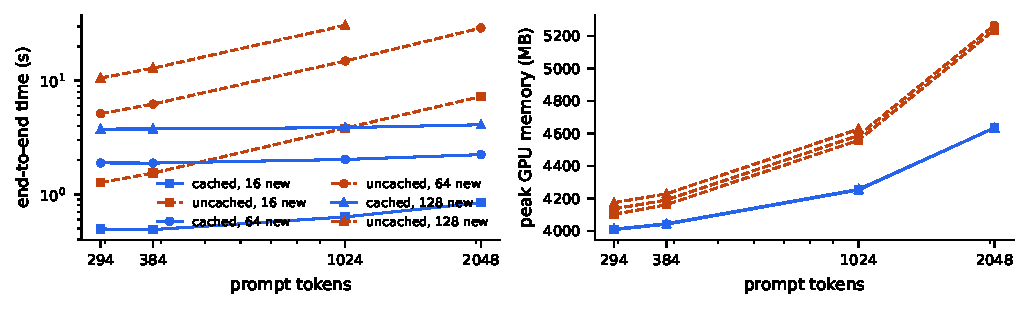
\includegraphics[width=0.85\textwidth]{figures/kv_cache}
\caption{KV-cached (solid) vs.\ uncached (dashed) greedy decoding on a T4: end-to-end time (left,
log-log) and peak GPU memory (right) as functions of prompt length for 16/64/128 new tokens.}
\label{fig:kv}
\end{figure*}

On the laptop CPU (fp32) the fine-tuned model needs about 12\,s per criterion in the application,
17\,s for the first criterion of a patient; prefix reuse saves the 234 shared prompt tokens
(of $\approx$360) for every subsequent criterion.

\subsection{Tiled attention}
\label{sec:res-attn}

\textbf{Correctness.} Against a float64 reference, both tiled variants (block 64 and 128) agree
with the reference and with PyTorch SDPA to within the precision of the input dtype on five shapes
including decode-style ($L_q{=}1$) and verification-style ($L_q{=}7$, $L_k{=}512$) causal cases:
maximum absolute error $9.8\cdot10^{-7}$ in fp32 and $1.6\cdot10^{-3}$ in fp16, with mean errors of
$4\cdot10^{-8}$ and $1.3\cdot10^{-4}$ (all implementations, including SDPA, show the same fp16 error,
which is the rounding of the fp16 output). In float64 the 64 unit tests agree with SDPA to
$10^{-10}$ for block sizes from 1 to 64, non-multiple lengths and padding masks. Used as the
attention backend of the real model, the tiled kernel reproduces the library's logits within
$2.6\cdot10^{-5}$ and identical generated tokens.

\textbf{Performance.} Fig.~\ref{fig:attn} shows the trade-off on the T4 (B=1, 12 heads, head
dimension 128, causal, fp16). Peak extra memory of the reference grows quadratically to 2.3\,GB at
4,096 tokens (the fp32 score matrix), while the tiled variants need 14--17\,MB, comparable to fused
SDPA (12\,MB): tiling achieves its purpose. Runtime tells the opposite story: tiled attention is
1.6--13$\times$ slower than our own reference and 65$\times$ slower than SDPA at 4,096 tokens
(254\,ms vs.\ 75\,ms vs.\ 3.9\,ms). The reason is that our tiling lives in Python: each of the
$(L/B)^2/2$ block pairs launches several small CUDA kernels (matrix products, exponentials,
rescaling) whose launch overhead dominates their arithmetic, every intermediate tile round-trips
through global memory, and larger blocks (128 vs.\ 64) are faster precisely because they launch fewer
kernels. A fused kernel such as FlashAttention performs the same online-softmax recurrence inside one
kernel, keeping tiles in on-chip shared memory and registers, so it gets the memory saving
\emph{and} the speed. The educational implementation demonstrates the algorithm and its memory
behaviour, not the speed.

\begin{figure*}[t]
\centering
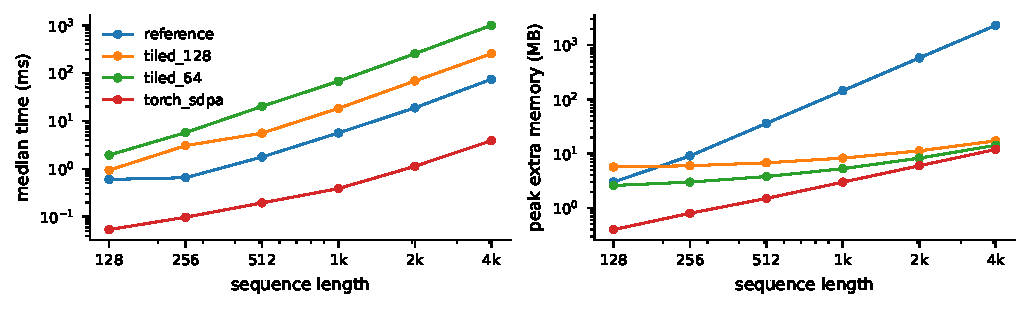
\includegraphics[width=0.85\textwidth]{figures/attention_perf}
\caption{Attention kernels on a T4 (fp16, B=1, H=12, d=128, causal): median runtime (left) and
peak extra GPU memory (right) vs.\ sequence length, both log scale.}
\label{fig:attn}
\end{figure*}

\subsection{Speculative decoding}
\label{sec:res-spec}

\textbf{Correctness.} Speculative decoding produced exactly the target's greedy tokens in all 96
benchmark configurations (two drafts $\times$ four draft lengths $\times$ 12 prompt/output lengths) and
on all 40 real screening prompts for both drafts. The unit tests additionally check equality for
$k\in\{1,3,5\}$ with a perfect draft, a noisy draft and a draft so noisy that fewer than half of
its tokens are accepted, which exercises the rejection and cache-rollback path, and stopping at EOS.

\textbf{Acceptance and speed.} Fine-tuning the draft on the same task raises acceptance on screening
prompts from 75.7\% to 92.6\% ($k=4$), and over longer generations from 61--84\% to 72--90\%
(Fig.~\ref{fig:spec}). Despite this, speculative decoding is not faster on the T4: on the 40
screening prompts it runs at 0.75$\times$ (base draft) and 0.90$\times$ (fine-tuned draft) of the
speed of KV-cached greedy, and over the length grid the speed-up ranges from 0.51 (base draft, $k=8$, short prompt) to 1.06.
With 128 new tokens and $k=4$, the fine-tuned draft gives 26.4--31.4 tokens/s against 31.2--34.2
for KV-cached greedy.

\textbf{Memory.} Speculative decoding keeps both models resident: 2.88\,GiB of fp16 target weights
plus 0.92\,GiB for the draft. In the benchmark both were loaded for every mode, so the measured peak
difference is the draft's own KV cache plus the activations of verifying $k{+}1$ tokens at once:
peak memory rises from 3.92 to 4.00\,GiB at a 294-token prompt and from 4.52 to 5.12\,GiB at 2,048
tokens ($k=4$, 128 new tokens). On the CPU-only laptop, where the models run in fp32, the draft adds
about 2\,GB, which is why the application checks free memory before loading it.

The explanation is the cost of a draft step relative to a target step. We measured single-token
decode steps of 23.6\,ms for the 0.5B draft and 28.5\,ms for the 1.5B target, a ratio $c=0.84$,
although the draft has a third of the parameters. At batch size 1 both models are dominated by
per-layer overhead (our decoder issues roughly 25 kernel launches per layer from Python, and the
draft has 24 layers against the target's 28) rather than by arithmetic or memory traffic. With
acceptance rate $\alpha$ and draft length $k$, the expected speed-up of
Leviathan et~al.~\cite{leviathan2023fast} is
$\frac{1-\alpha^{k+1}}{(1-\alpha)(ck+1)}$; with $c=0.84$ it predicts 1.05, 1.00 and 0.89 for
$\alpha=0.93$ and $k=2, 4, 8$, and 0.70 for $\alpha=0.75$, $k=4$, matching the measured 0.90 and
0.75 on screening prompts. Short outputs make things worse: a screening answer has only
$\approx$15 tokens, so the fixed cost of prefilling the draft model is amortized over very few
tokens. Speculative decoding pays off when $c$ is small, e.g.\ with a fused inference engine, a much
smaller draft relative to the target (a 7B target with a 0.5B draft) or memory-bound larger
batches, none of which applies to this deployment.

\begin{figure*}[t]
\centering
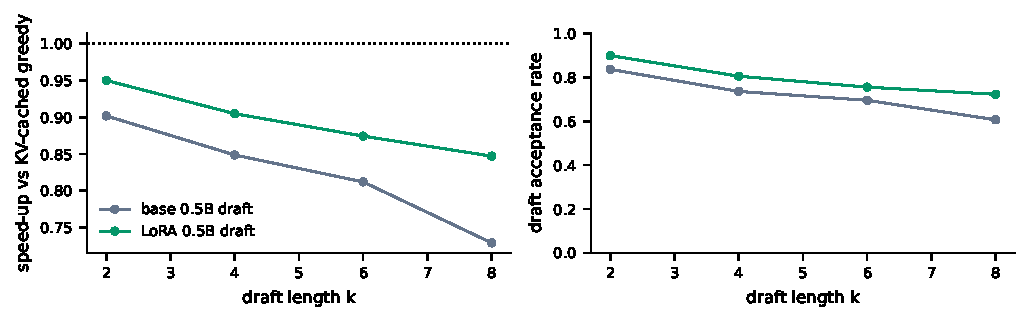
\includegraphics[width=0.85\textwidth]{figures/speculative}
\caption{Speculative decoding on a T4 with the base and the fine-tuned 0.5B draft, averaged over
the four prompt lengths at 128 new tokens: speed-up vs.\ KV-cached greedy (left; $<1$ is a
slowdown) and draft acceptance rate (right) as functions of the draft length $k$.}
\label{fig:spec}
\end{figure*}

\subsection{Application}
\label{sec:res-app}

Fig.~\ref{fig:app} shows the application screening a validation patient. Each criterion result
links its label to the highlighted note sentences, shows the evidence-only explanation and flags,
and the expert label when an example from the validation split is loaded. The benchmark page runs
the four decoding implementations on the current prompt and reports their timings, token equality
and acceptance; invalid inputs (empty note, empty or malformed criteria, prompts over the token
limit, unknown modes, malformed NCT IDs) are rejected with specific messages, and a failing criterion
does not abort the rest of a screening. Saved reports carry the model, adapter, decoding settings and
creation time.

\begin{figure*}[t]
\centering
\begin{minipage}[t]{0.49\textwidth}\vspace{0pt}
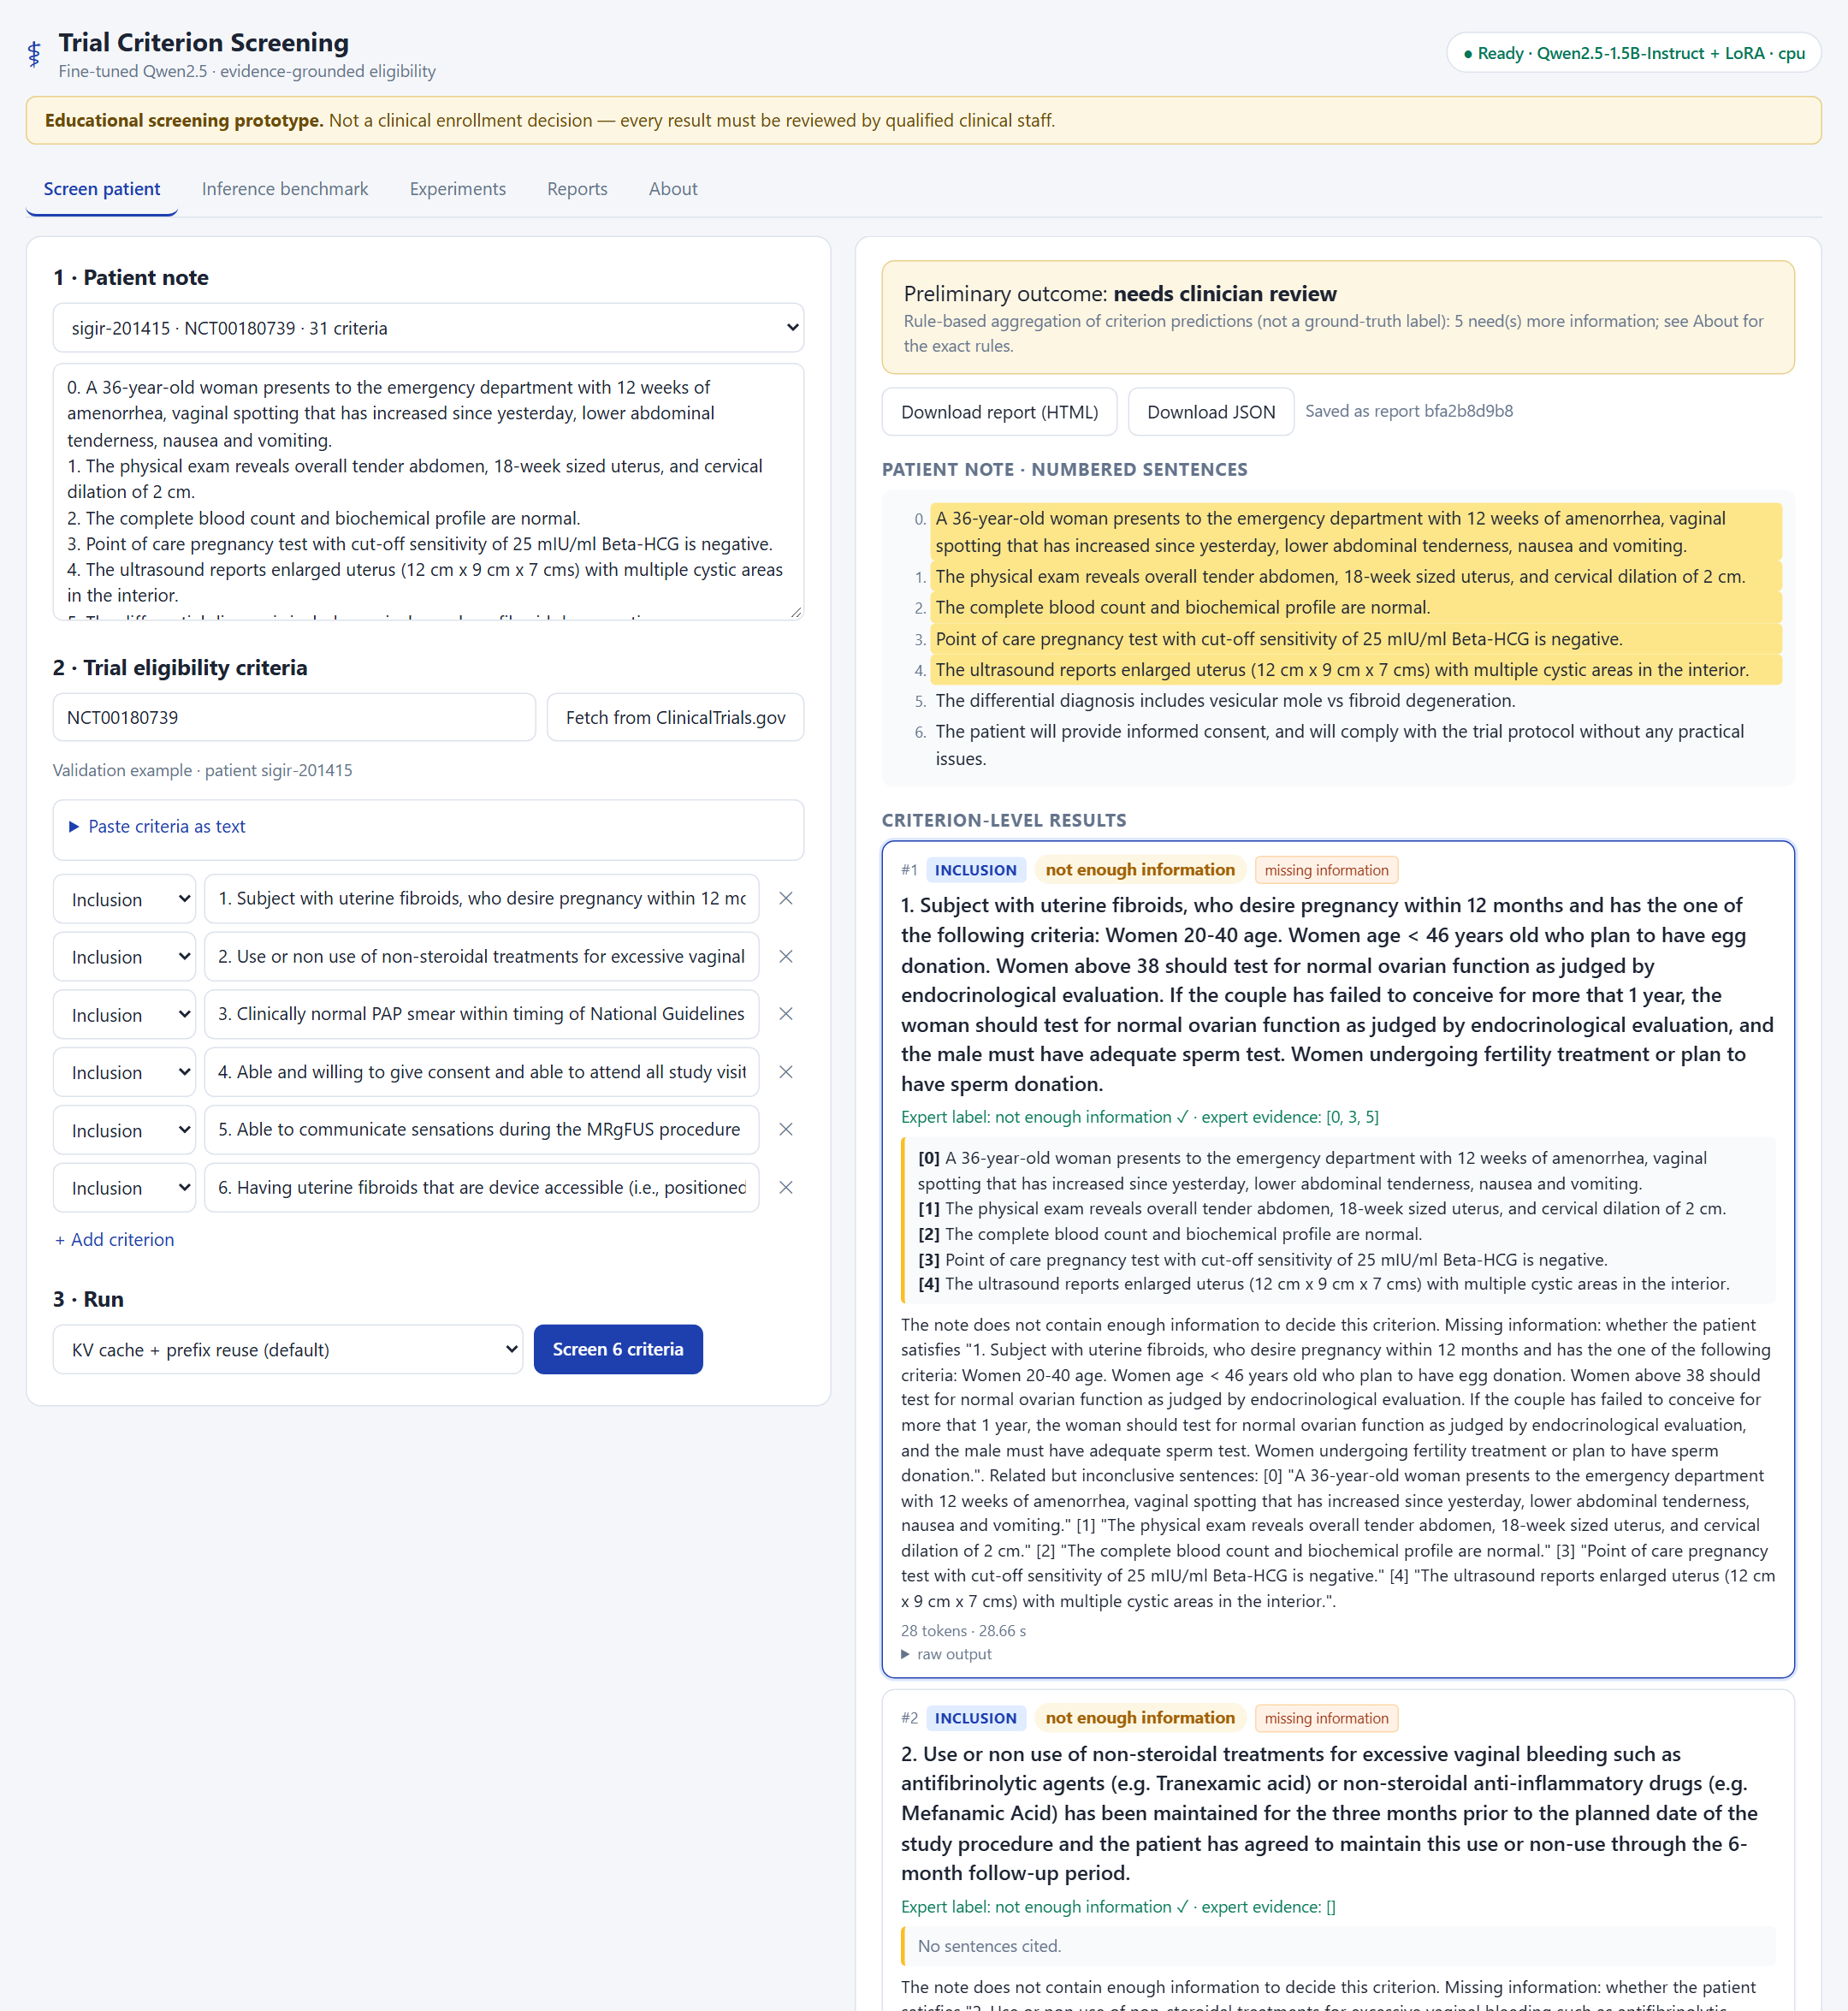
\includegraphics[width=\linewidth]{figures/screens/screen_top}
\end{minipage}\hfill
\begin{minipage}[t]{0.49\textwidth}\vspace{0pt}
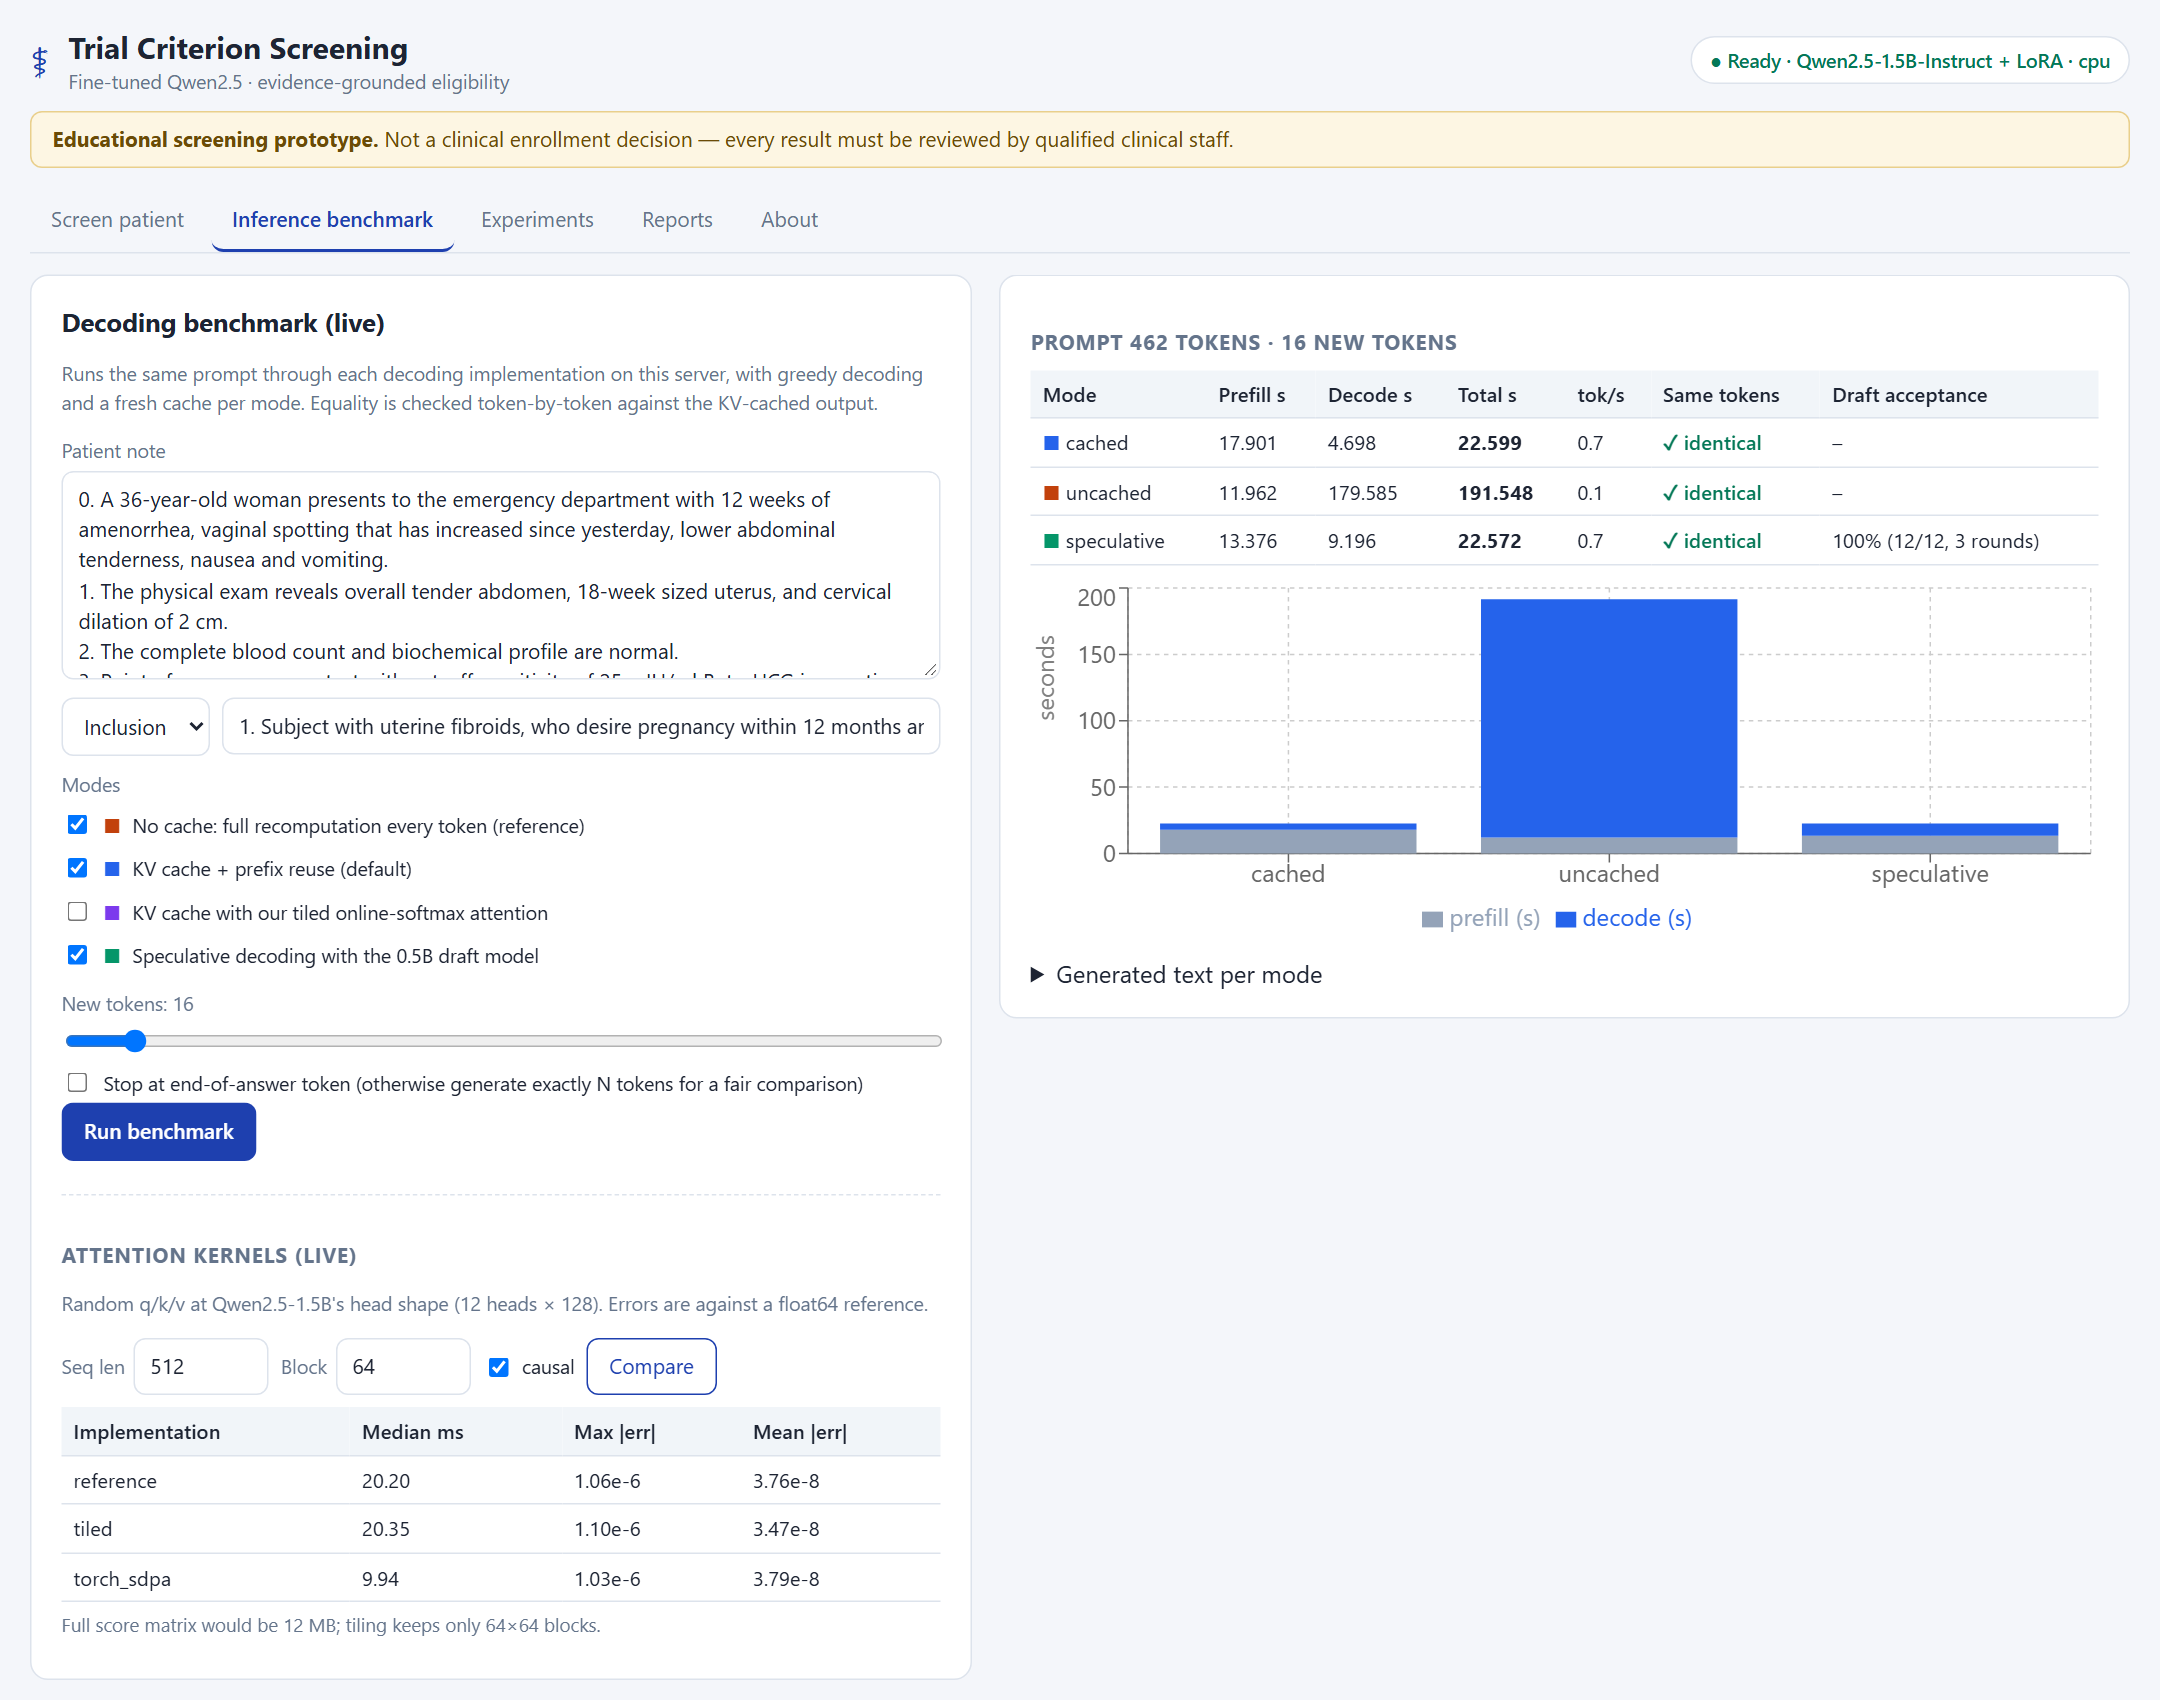
\includegraphics[width=\linewidth]{figures/screens/benchmark_crop}
\end{minipage}
\caption{The application running in Docker on the CPU-only laptop with the published adapter. Left:
screening six criteria of a validation patient; the selected result's cited sentences are highlighted
in the numbered note, the explanation quotes them, and the expert label is shown for comparison
(all six match). Right: the live benchmark page comparing KV-cached, uncached and speculative
decoding on the same prompt (identical tokens, 100\% draft acceptance; uncached decoding is
8.5$\times$ slower), and the live attention-kernel accuracy check.}
\label{fig:app}
\end{figure*}

\section{Limitations}
\label{sec:limitations}

\textbf{Data size and label noise.} The benchmark has 53 patients; the test split holds 206
criteria from 8 patients, no \emph{excluded} example, and only 3--7 examples of several other
classes, so per-class test figures have wide uncertainty and the test set is dominated by a few
patients and trials (one patient contributes 14 of the 25 largest-group errors). The error analysis
shows that annotators applied the \emph{not excluded} versus \emph{not enough information}
distinction inconsistently for conditions the note does not mention; part of the measured error
reflects this ambiguity rather than model failure, and conversely the model has learned a convention
(absence $\Rightarrow$ not excluded) that a screening tool should not apply blindly.

\textbf{Model capacity and reasoning.} A 1.5B model does not perform the clinical inferences and
counting that some criteria require (Table~\ref{tab:errors}), and it essentially never predicts the
rarest classes. Explanations are assembled from cited sentences rather than generated, which avoids
hallucinated rationales but cannot express the reasoning linking evidence to label. The model judges
each criterion independently and ignores compound logic across criteria.

\textbf{Selection and evaluation.} Model selection used a validation set too small to separate the
variants statistically; the chosen configuration's advantage is not significant, although seed
repeats show it is stable. We evaluated a single dataset; generalization to real clinical notes,
which are longer, noisier and not pre-split into sentences, is untested. The application's sentence
splitter for unseen notes is rule-based and may split or merge sentences differently from the
dataset's annotation.

\textbf{Inference implementations.} Our decoders run at batch size 1 and do not implement paged or
quantized caches. The tiled attention is an educational Python implementation that saves memory but
is much slower than fused kernels. Speculative decoding gives no speed-up in our setting because the
draft is not cheap enough relative to the target at batch size 1; we did not evaluate larger target
models, where it would be expected to help. Timings were measured on one T4 and one laptop CPU and
include Kaggle's shared-infrastructure variability.

\textbf{Clinical use.} The system is an educational screening prototype. It has not been validated
clinically, is not a medical device, and must not be used for enrollment decisions; every result
requires review by qualified staff.

\section{Conclusion}
\label{sec:conclusion}

A 1.5B open-weight decoder, adapted with LoRA on 602 expert-labelled criteria in under 14 minutes of
free GPU time, judges individual trial eligibility criteria with held-out accuracy 0.748, macro-F1
0.569 and evidence micro-F1 0.513, up from near-zero for the untuned model under the same prompt,
and its published adapter reproduces exactly on a CPU-only laptop. The model is reliable on the
frequent classes but defers to \emph{not enough information} where experts draw clinical
inferences, never predicts the rarest classes, and has inherited the annotators' inconsistent
treatment of unmentioned exclusion conditions; the application therefore surfaces such absence-based
judgements for verification instead of presenting them as facts.

On the inference side, our explicit KV cache is token-identical to recomputation in fp32 and raises
throughput up to 13$\times$ at long prompts; the only fp16 disagreements trace back to exact
top-2 ties under different kernels. Tiled online-softmax attention matches exact attention to float
precision while cutting attention memory from 2.3\,GB to 17\,MB at 4,096 tokens, but is slower than
fused kernels when written in Python. Greedy speculative decoding is exactly output-preserving and a
fine-tuned draft reaches 93\% acceptance, yet the measured draft/target cost ratio of 0.84 at batch
size 1 predicts and explains the absence of a speed-up. Future work includes larger targets with the
same draft, consistency-aware training labels for missing information, generated but evidence-checked
explanations, and evaluation on real clinical notes.


\bibliographystyle{IEEEtran}
\bibliography{references}

\appendices
\section{Use of AI Assistance}
\label{app:ai}
An AI coding assistant (Anthropic's Claude, used through Claude Code) was used throughout this
project: to draft and refactor source code (data pipeline, training and evaluation scripts, the
decoder, attention and speculative-decoding implementations, the FastAPI backend and React
front end, Docker configuration), to write tests and benchmark scripts, to drive the Kaggle jobs, and
to draft this report. All numbers in the report come from logged runs in the repository
(\code{results/}); none were produced or edited by the assistant without a corresponding run.
Reused library code (PyTorch, Transformers, PEFT, scikit-learn, FastAPI, React, Recharts) is used
through public APIs; our own implementations of KV-cached decoding, tiled attention and speculative
decoding are verified by the automated tests described in Section~\ref{sec:results}. The author
reviewed, executed and is responsible for the complete submission.


\end{document}
